\subsection{Застосування алгоритму Бойкова-Колмогорова}

Окремо Б-К алгоритм не є корисним для детекції рухомих об'єктів. У даній роботі
використано метод \cite{bib:pavliuk_krygin}, який у свою чергу використовує алгоритм Б-К
для пошуку мінімального розрізу на графі, що дозволяє знаходити
маску рухомих об'єктів та має можливість налаштовувати ступінь взаємодії сусідніх
пікселів.
\begin{definition}
	Маскою рухомих об'єктів кадру \(F^{i}\) будемо називати бінарне
	зображення \(B^{i}:P \rightarrow \left\{ 0,1 \right\}\), де тим
	пікселям, в яких на відповідному кадрі \(F^{i}\) було помічено рух,
	відповідає одиниця, а іншим відповідає нуль.
\end{definition}

Для обраного користувачем
кроку $s \in \mathbb{N}$ на двох кадрах \(F^{i}\) і \(F^{i + s}\) рухомі об'єкти
являють собою підмножину пікселів, колір яких було змінено більше, ніж
на певне значення, з урахуванням зміни кольорів у сусідніх пікселях.
Тобто, якщо рухомий об'єкт складається з одного пікселя, його рух може
бути проігнорованим в залежності від обраних користувачем налаштувань,
про які йдеться мова далі; аналогічно, якщо рухомий об'єкт на кадрі
містить нерухомі «дірки» (пікселі, де колір не змінився), вони можуть
вважатися частиною рухомого об'єкту.

\begin{figure}[H]
	\centering
	\subfloat[Попередній кадр $F^i$]{
		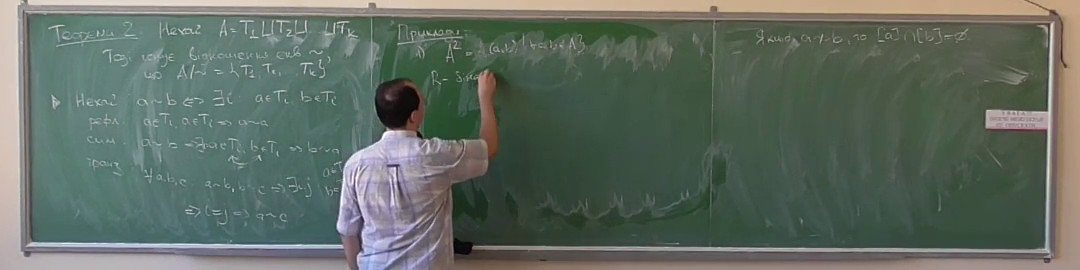
\includegraphics[width=0.55\textwidth]{images/prev_frame}
		\label{fig:yakovlev_discrete_math:bk_examples:a}
	}\\
	\subfloat[Поточний кадр $F^{i+s}$]{
		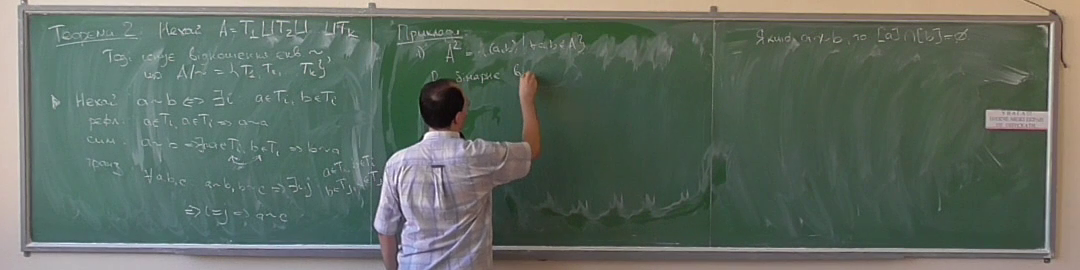
\includegraphics[width=0.55\textwidth]{images/next_frame}
		\label{fig:yakovlev_discrete_math:bk_examples:b}
	}\\
	\subfloat[Інвертована різниця $F^i$ і $F^{i+s}$]{
		
\includegraphics[width=0.55\textwidth]{images/inv_diff}
		\label{fig:yakovlev_discrete_math:bk_examples:c}
	}\\
	\subfloat[Маска рухомих об'єктів на кадрі $F^{i+s}$]{
		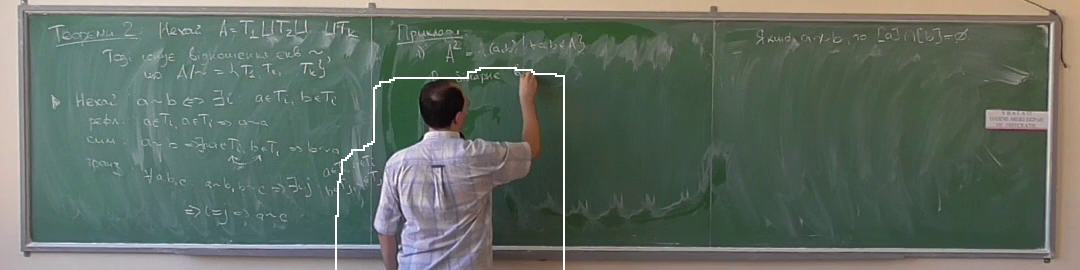
\includegraphics[width=0.55\textwidth]{images/next_with_mask}
		\label{fig:yakovlev_discrete_math:bk_examples:d}
	}
	\caption{Процес створення маски рухомих об'єктів з відео \cite{video:mmzi:yakovlev_discrete_math}
		\label{fig:yakovlev_discrete_math:bk_examples}
	}
\end{figure}

Для того, щоб отримати маску рухомих об'єктів, які можуть перекривати дошку, ми
беремо кадри \(F^{i}\) та \(F^{i + s}\) (рис.
\subref{fig:yakovlev_discrete_math:bk_examples:a},
\subref{fig:yakovlev_discrete_math:bk_examples:b}) та для
кожної пари кольорів пікселів \(p\) з однаковими координатами знаходимо
модуль \(D_{p}^{i} = \left| F_{p}^{i} - F_{p}^{i + s} \right|\) різниці
інтенсивностей (рис. \ref{fig:yakovlev_discrete_math:bk_examples:c}). Зображення \(D^{i}\) подаємо на вхід
Б-К алгоритму.

Знайдемо маску $B^{i}:P \rightarrow \{0,1\}$ рухомих
об'єктів для кадрів \(F^{i}\) і \(F^{i + s}\).
Введемо функції.
\begin{align*}
	 & q_{p}(B_{p}^{i}) =
	\begin{cases}
		\alpha D_{p}^{i}, & \textit{якщо} \quad B_{p}^{i} = 0,  \\
		255 - D_{p}^{i},  & \textit{якщо} \quad B_{p}^{i} = 1 ,
	\end{cases}     \\
	 & g(B_{p}^{i},B_{p'}^{i}) = \beta|B_{p}^{i} - B_{p'}^{i}|,
\end{align*}
де \(\alpha\) та \(\beta\)~---~параметри згладжування маски, що задаються
користувачем інформаційної технології. Позначимо множину
$\Gamma \subset P^{2}$ сусідніх пікселів. У даній роботі сусідніми до
пікселя \(p \in P\) вважаються пікселі з множини
\(\left\{ \left( p_{x + 1},p_{y} \right),\left( p_{x},p_{y + 1} \right) \right\} \cap P\).
Сформулюємо пошук маски \(B^{i}\) у вигляді задачі мінімізації виразу
\begin{equation*}
	E\left( B_{p}^{i} \right) = \sum_{p \in P}^{}{q_{{p\ }}( B_{p}^{i}) +}\sum_{(p,p') \in \Gamma}^{}g(B_{p}^{i},B_{p'}^{i}).
\end{equation*}
На виході отримуємо маску \(B_{p}^{i}\) рухомих об'єктів (рис.
\ref{fig:yakovlev_discrete_math:bk_examples:d}).
Її ми використовуємо, щоб не переносити на фінальне зображення ті
пікселі, на яких було помічено рух, адже зміна яскравості пікселя
виникає не тільки під час створення напису, а й під час тимчасового
затуляння дошки.
